\documentclass[oneside,openany,headings=optiontotoc,11pt,numbers=noenddot]{scrreprt}

\usepackage[a4paper]{geometry}
\usepackage[utf8]{inputenc}
\usepackage[T1]{fontenc}
\usepackage{lmodern}
\usepackage[ngerman]{babel}
\usepackage{ngerman}

\usepackage[onehalfspacing]{setspace}

\usepackage{fancyhdr}
\usepackage{fancybox}

\usepackage{rotating}
\usepackage{varwidth}

%Struktogramme
\usepackage[german,curves]{struktex}

\usepackage{pdflscape}
\usepackage{changepage}
\usepackage{graphicx}
\usepackage[bottom]{footmisc}
\usepackage{transparent}
\usepackage{graphbox}
\graphicspath{
	{Pics/PDFs/}
	{Pics/JPGs/}
	{Pics/PNGs/}
}
\usepackage{caption}
\usepackage{wrapfig}
\usepackage{marginnote}
\usepackage{tabularx}
\usepackage{dashrule}
\usepackage{soulutf8}
\usepackage{hhline}
%arydshln suppresses vertical lines in table
%\usepackage{arydshln}
\usepackage{multirow}
\usepackage{enumerate}
\usepackage[hidelinks]{hyperref}
\usepackage{listings}

\usepackage[table]{xcolor}
\usepackage{array}
\usepackage{enumitem,amssymb,amsmath}
\usepackage{interval}
\usepackage{cancel}
\usepackage{stmaryrd}
\usepackage{wasysym}
\usepackage{polynom}
\usepackage{diagbox}
\usepackage{dashrule}
\usepackage{framed}
\usepackage{mdframed}
\usepackage{karnaugh-map}
\usepackage{pdfpages}

\usepackage{blindtext}

\usepackage{eso-pic}

\usepackage{amssymb}
\usepackage{eurosym}

\usepackage[pages=some]{background}
\pagestyle{headings}
\renewcommand{\headrulewidth}{0.2pt}
\renewcommand{\footrulewidth}{0.2pt}
\newcommand*{\underdownarrow}[2]{\ensuremath{\underset{\overset{\Big\downarrow}{#2}}{#1}}}
\setlength{\fboxsep}{5pt}
\newcommand{\explainBelow}[3]{\underbrace{#1}_{\parbox{\widthof{#3}}{\footnotesize\raggedright #2}}}
\newcommand{\explainAbove}[3]{\overbrace{#1}^{\parbox{\widthof{#3}}{\footnotesize\raggedright #2}}}
\newcommand\footnoteref[1]{\protected@xdef\@thefnmark{\ref{#1}}\@footnotemark}


% Codestyle defined
\definecolor{codegreen}{rgb}{0,0.6,0}
\definecolor{codegray}{rgb}{0.5,0.5,0.5}
\definecolor{codepurple}{rgb}{0.58,0,0.82}
\definecolor{backcolour}{rgb}{0.95,0.95,0.92}
\definecolor{deepgreen}{rgb}{0,0.5,0}
\definecolor{darkblue}{rgb}{0,0,0.65}
\definecolor{mauve}{rgb}{0.40, 0.19,0.28}
\colorlet{exceptioncolour}{yellow!50!red}
\colorlet{commandcolour}{blue!60!black}
\colorlet{numpycolour}{blue!60!green}
\colorlet{specmethodcolour}{violet}

%Neue Spaltendefinition
\newcolumntype{L}[1]{>{\raggedright\let\newline\\\arraybackslash\hspace{0pt}}m{#1}}
\newcolumntype{M}{>{\centering\arraybackslash}X}
\newcommand{\cmnt}[1]{\ignorespaces}
%Textausrichtung ändern
\newcommand\tabrotate[1]{\rotatebox{90}{\raggedright#1\hspace{\tabcolsep}}}

%Intervall-Konfig
\intervalconfig {
	soft open fences
}

%Bash
\lstdefinestyle{BashInputStyle}{
	language=bash,
	basicstyle=\small\sffamily,
	backgroundcolor=\color{backcolour},
	columns=fullflexible,
	backgroundcolor=\color{backcolour},
	breaklines=true,
}
%Java
\lstdefinestyle{JavaInputStyle}{
	language=Java,
	backgroundcolor=\color{backcolour},
	aboveskip=1mm,
	belowskip=1mm,
	showstringspaces=false,
	columns=flexible,
	basicstyle={\footnotesize\ttfamily},
	numberstyle={\tiny},
	numbers=none,
	keywordstyle=\color{purple},,
	commentstyle=\color{deepgreen},
	stringstyle=\color{blue},
	emph={out},
	emphstyle=\color{darkblue},
	emph={[2]rand},
	emphstyle=[2]\color{specmethodcolour},
	breaklines=true,
	breakatwhitespace=true,
	tabsize=2,
}
%Python
\lstdefinestyle{PythonInputStyle}{
	language=Python,
	alsoletter={1234567890},
	aboveskip=1ex,
	basicstyle=\footnotesize,
	breaklines=true,
	breakatwhitespace= true,
	backgroundcolor=\color{backcolour},
	commentstyle=\color{red},
	otherkeywords={\ , \}, \{, \&,\|},
	emph={and,break,class,continue,def,yield,del,elif,else,%
		except,exec,finally,for,from,global,if,import,in,%
		lambda,not,or,pass,print,raise,return,try,while,assert},
	emphstyle=\color{exceptioncolour},
	emph={[2]True,False,None,min},
	emphstyle=[2]\color{specmethodcolour},
	emph={[3]object,type,isinstance,copy,deepcopy,zip,enumerate,reversed,list,len,dict,tuple,xrange,append,execfile,real,imag,reduce,str,repr},
	emphstyle=[3]\color{commandcolour},
	emph={[4]ode, fsolve, sqrt, exp, sin, cos, arccos, pi,  array, norm, solve, dot, arange, , isscalar, max, sum, flatten, shape, reshape, find, any, all, abs, plot, linspace, legend, quad, polyval,polyfit, hstack, concatenate,vstack,column_stack,empty,zeros,ones,rand,vander,grid,pcolor,eig,eigs,eigvals,svd,qr,tan,det,logspace,roll,mean,cumsum,cumprod,diff,vectorize,lstsq,cla,eye,xlabel,ylabel,squeeze},
	emphstyle=[4]\color{numpycolour},
	emph={[5]__init__,__add__,__mul__,__div__,__sub__,__call__,__getitem__,__setitem__,__eq__,__ne__,__nonzero__,__rmul__,__radd__,__repr__,__str__,__get__,__truediv__,__pow__,__name__,__future__,__all__},
	emphstyle=[5]\color{specmethodcolour},
	emph={[6]assert,range,yield},
	emphstyle=[6]\color{specmethodcolour}\bfseries,
	emph={[7]Exception,NameError,IndexError,SyntaxError,TypeError,ValueError,OverflowError,ZeroDivisionError,KeyboardInterrupt},
	emphstyle=[7]\color{specmethodcolour}\bfseries,
	emph={[8]taster,send,sendMail,capture,check,noMsg,go,move,switch,humTem,ventilate,buzz},
	emphstyle=[8]\color{blue},
	keywordstyle=\color{blue}\bfseries,
	rulecolor=\color{black!40},
	showstringspaces=false,
	stringstyle=\color{deepgreen}
}

\lstset{literate=%
	{Ö}{{\"O}}1
	{Ä}{{\"A}}1
	{Ü}{{\"U}}1
	{ß}{{\ss}}1
	{ü}{{\"u}}1
	{ä}{{\"a}}1
	{ö}{{\"o}}1
}

% Neue Klassenarbeits-Umgebung
\newenvironment{worksheet}[3]
% Begin-Bereich
{
	\newpage
	\sffamily
	\setcounter{page}{1}
	\ClearShipoutPicture
	\AddToShipoutPicture{
		\put(55,761){{
				\mbox{\parbox{385\unitlength}{\tiny \color{codegray}BBS I Mainz, #1 \newline #2
						\newline #3
					}
				}
			}
		}
		\put(455,761){{
				\mbox{\hspace{0.3cm}
\includegraphics[width=0.2\textwidth]{../../logo.pdf}}
			}
		}
	}
}
% End-Bereich
{
	\clearpage
	\ClearShipoutPicture
}

\geometry{left=2.50cm,right=2.50cm,top=3.00cm,bottom=1.00cm,includeheadfoot}

\begin{document}
	\begin{worksheet}{Höhere Berufsfachschule IT-Systeme}{Grundstufe - Mathematik}{Lernabschnitt 1: Lineare Funktionen - Übung}
		\noindent
		\LARGE Wohnungen in Mainz\\
		\normalsize
		\noindent
		Die Entwicklung der Anzahl der Wohnungen in Mainz lässt sich durch die folgende Tabelle grob darstellen:\\
		\par\noindent
		\begin{tabularx}{\columnwidth}{|X|l|l|M}
			\cline{1-3}
			\(x\) (in Jahren; \(0 = 2000\)) & 0 & 10 & \multirow{2}{*}{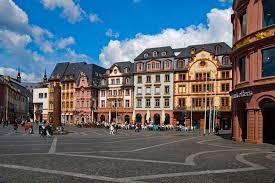
\includegraphics[width=0.15\textwidth]{../99_Bilder/mz.jpg}}\\
			\cline{1-3}
			\(y\) (Wohnungen in Tausend) & 95 & 101 &\\
			\cline{1-3}
		\end{tabularx}\\
		\begin{framed}
			\noindent
			\small{\color{codegray}Leitfrage:}\\
			
\includegraphics[width=0.1\textwidth]{../../empty.jpg}\\
		\end{framed}
		\begin{framed}
			\noindent
			\small{\color{codegray}Berechnung:}\\
			
\includegraphics[width=0.2\textwidth]{../../empty.jpg}\\
			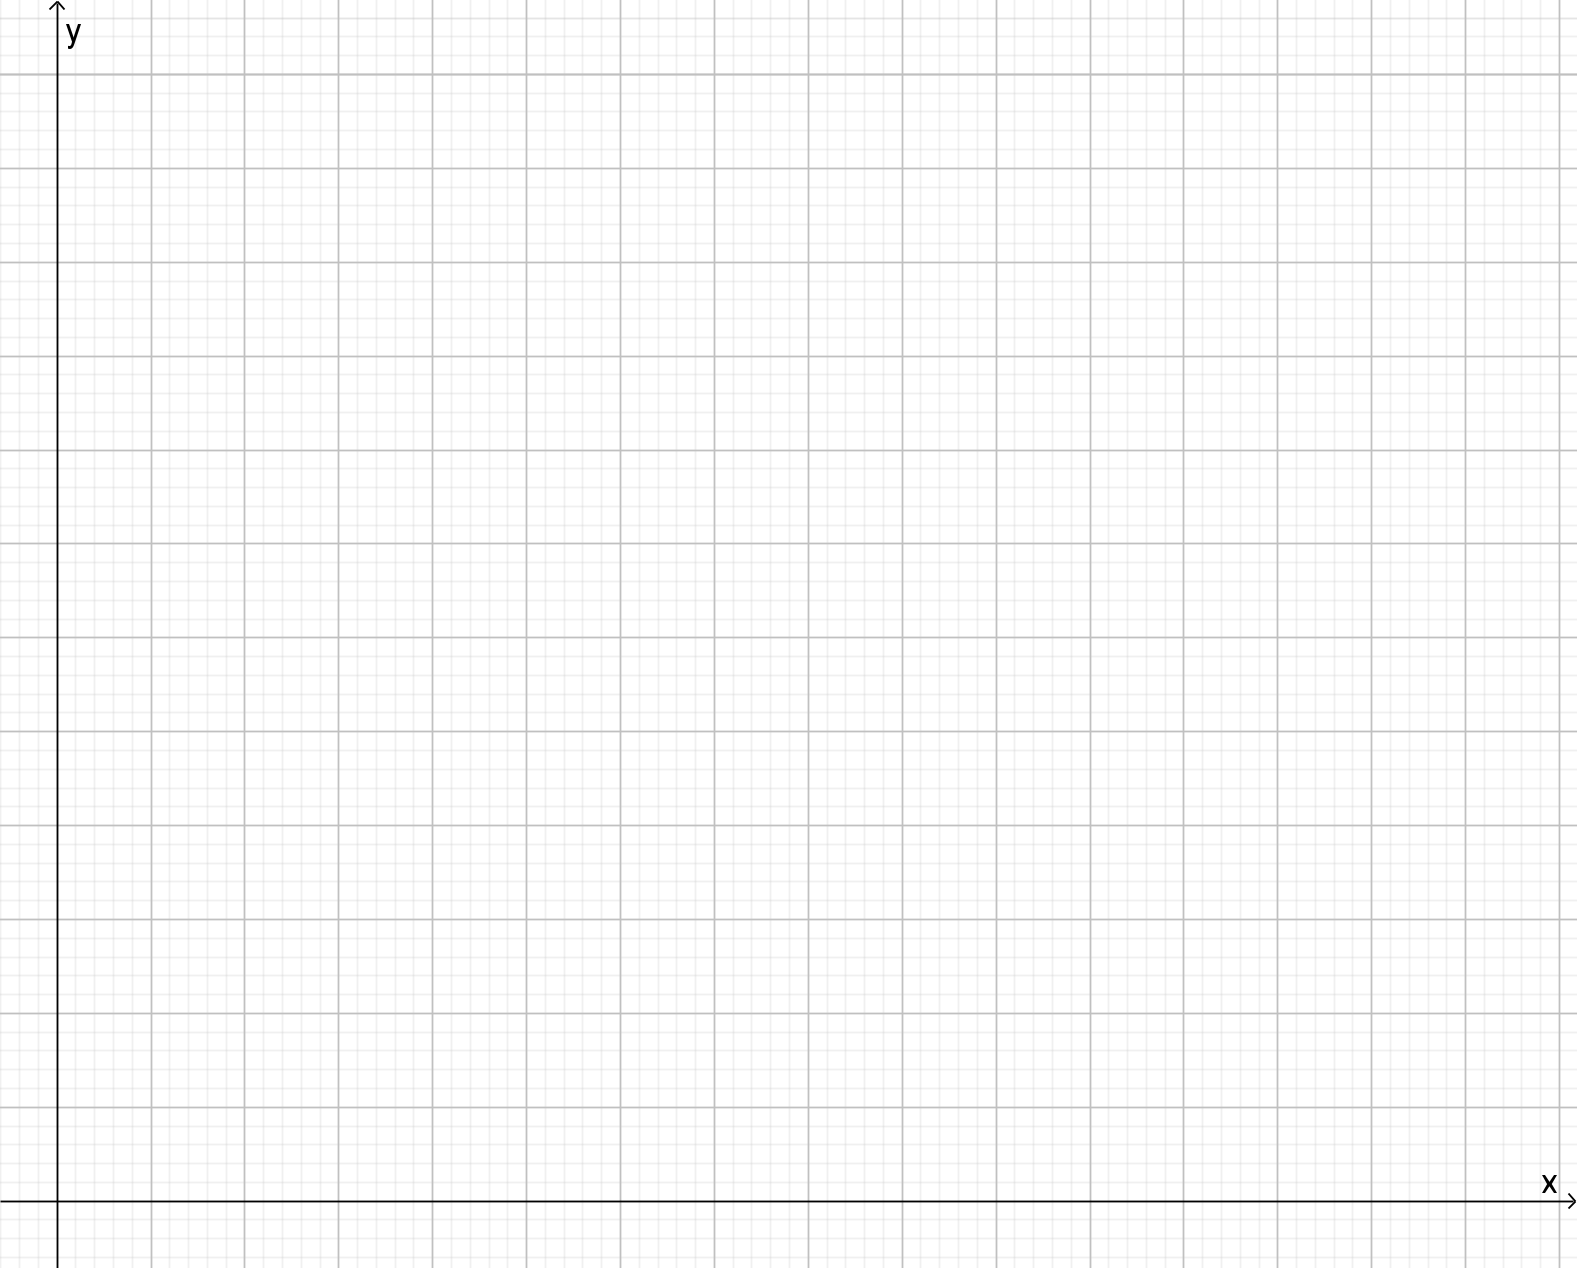
\includegraphics[width=0.86\textwidth]{../99_Bilder/KoordLeer.png}
		\end{framed}
		\normalsize
		\begin{framed}
			\noindent
			Interpretation der Steigung \(m\):\\
			
\includegraphics[width=0.1\textwidth]{../../empty.jpg}\\
		\end{framed}
		\par\bigskip\noindent
		\begin{framed}
			\noindent
			Es ist bekannt, dass die Anzahl der Schüler in der Mittelstufe von \(13.300 (2006)\) auf \(11.800 (2013)\) gesunken ist.\\
			Stellen Sie eine Gleichung auf, die diese Entwicklung modelliert.\\
			\par\noindent
			Bestimmen Sie die Anzahl der Schüler nach 12, 15 und nach 20 Jahren.
		\end{framed}
		\begin{framed}
			
\includegraphics[width=0.8\textwidth]{../../empty.jpg}
		\end{framed}
		\newpage
		
		%Blatt 2
		\setcounter{page}{1}
		\noindent
		\LARGE Mitgliedsbeiträge\\
		\normalsize
		\noindent
		\begin{tabularx}{\textwidth}{Xr}
			Der Vorstand einer großen Fitness-Studio Kette überlegt, welche Mitgliedsbeiträge im nächsten Jahr verlangt werden soll. Dabei wollen sie ein Unterscheidung von Erwachsenen und Jugendlichen machen. & \multirow{2}{*}{
\includegraphics[width=0.15\textwidth,align=b]{../99_Bilder/sporty.jpg}}\\
			Insgesamt benötigt die Studio-Kette einen Erlös von \(28.800\)\euro{}. & \\
			Im Studio sind 120 Erwachsene und 50 Jugendliche Mitglieder angemeldet.
		\end{tabularx}
		\begin{framed}
			\noindent
			\small{\color{codegray}Leitfrage:}\\
			
\includegraphics[width=0.1\textwidth]{../../empty.jpg}\\
		\end{framed}
		\begin{framed}
			\noindent
			\small{\color{codegray}Berechnung:}\\
			
\includegraphics[width=0.2\textwidth]{../../empty.jpg}\\
			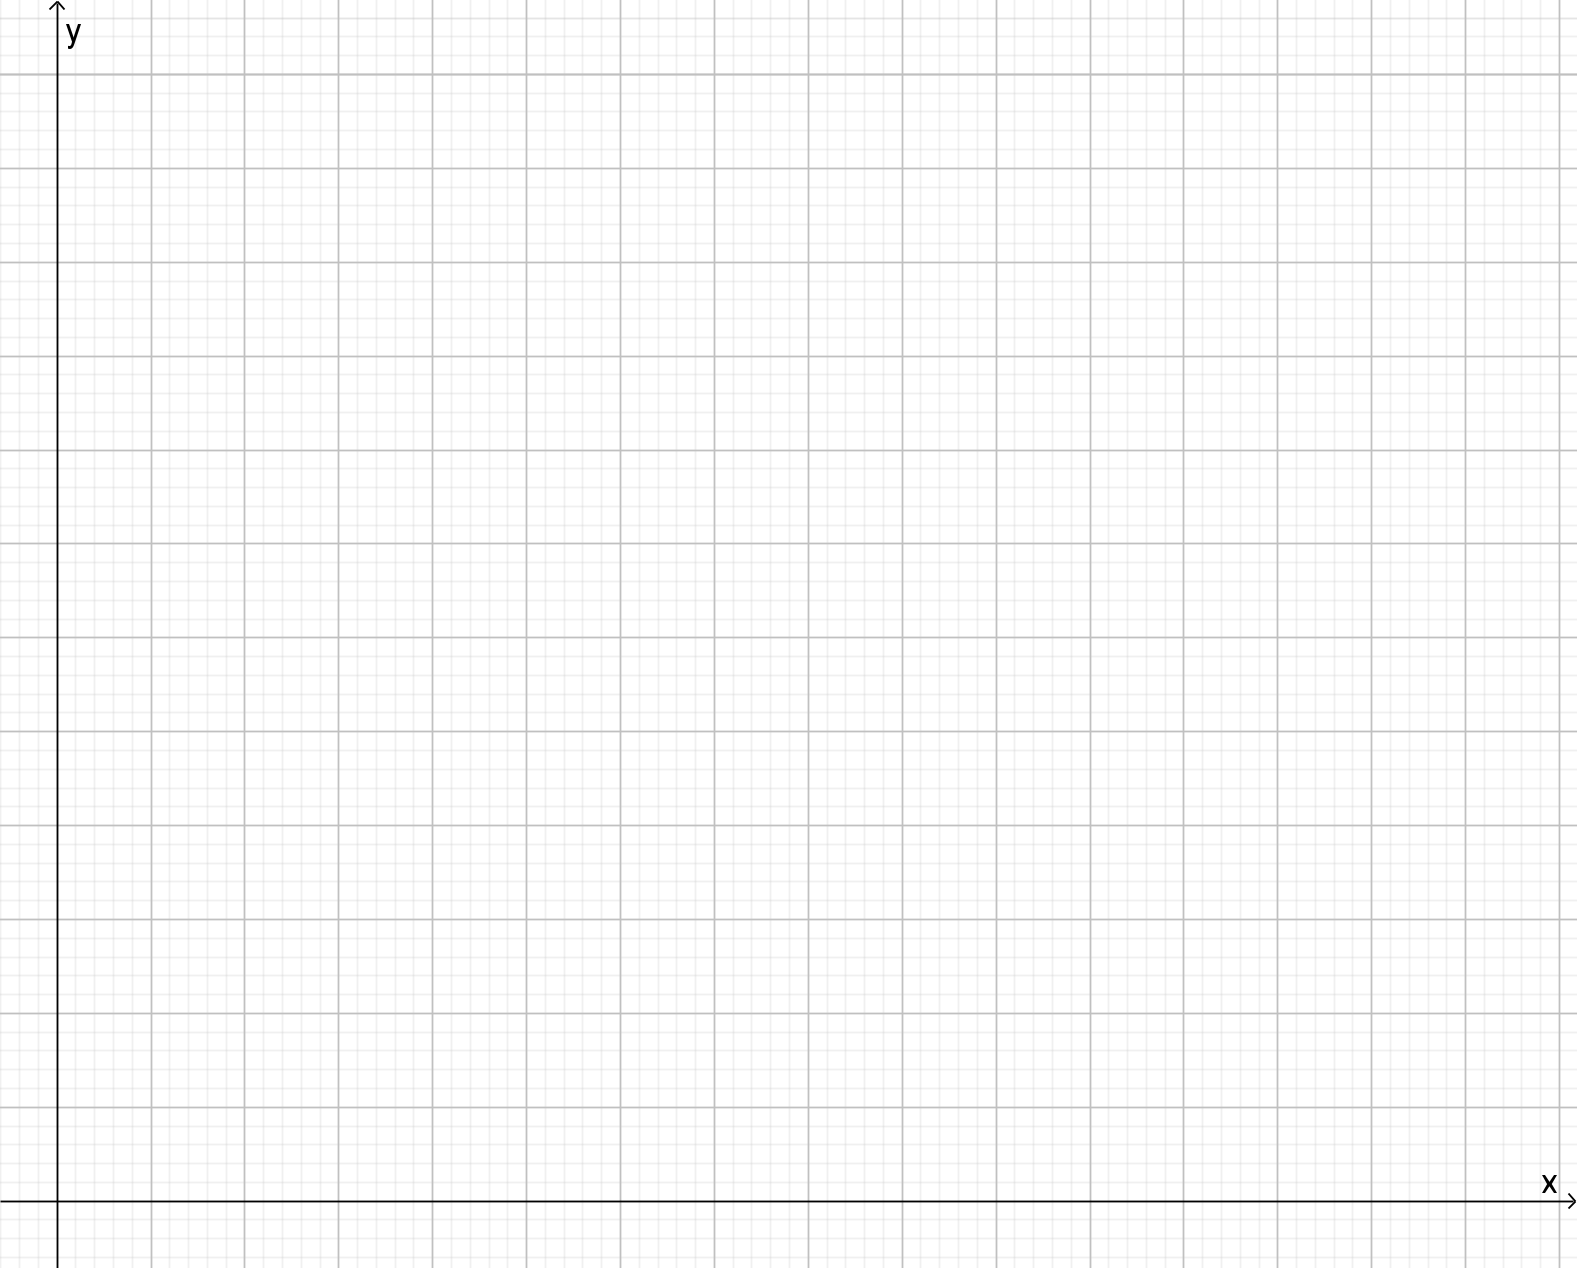
\includegraphics[width=0.86\textwidth]{../99_Bilder/KoordLeer.png}
		\end{framed}
		\normalsize
		\newpage
		\begin{framed}
			\noindent
			Die Entwicklung der Schüler an Mainzer Gymnasien wird durch die mit \(y=0,1x+3\) gegebenen Funktion modelliert. Dabei ist \(x\) in Jahren gegeben und \(x = 0\) entspricht dem Jahr \(2005\). Der Wert \(y\) ist in Tausend Schüler angegeben.
			\begin{itemize}
				\item[(a)] Zeichnen Sie den Graphen der Funktion \underline{ohne eine Wertetabelle} anzulegen!
				\item[(b)] Interpretieren Sie die Steigung und den y-Achsenabschnitt im Hinblick auf die Situation.
				\item[(c)] Berechnen Sie den Zeitpunkt, ab dem laut Modell über \(4000\) Schüler an Mainzer Gymnasien sind.\\
				Beurteilen sie Ihr Ergebnis kritisch!
			\end{itemize}
			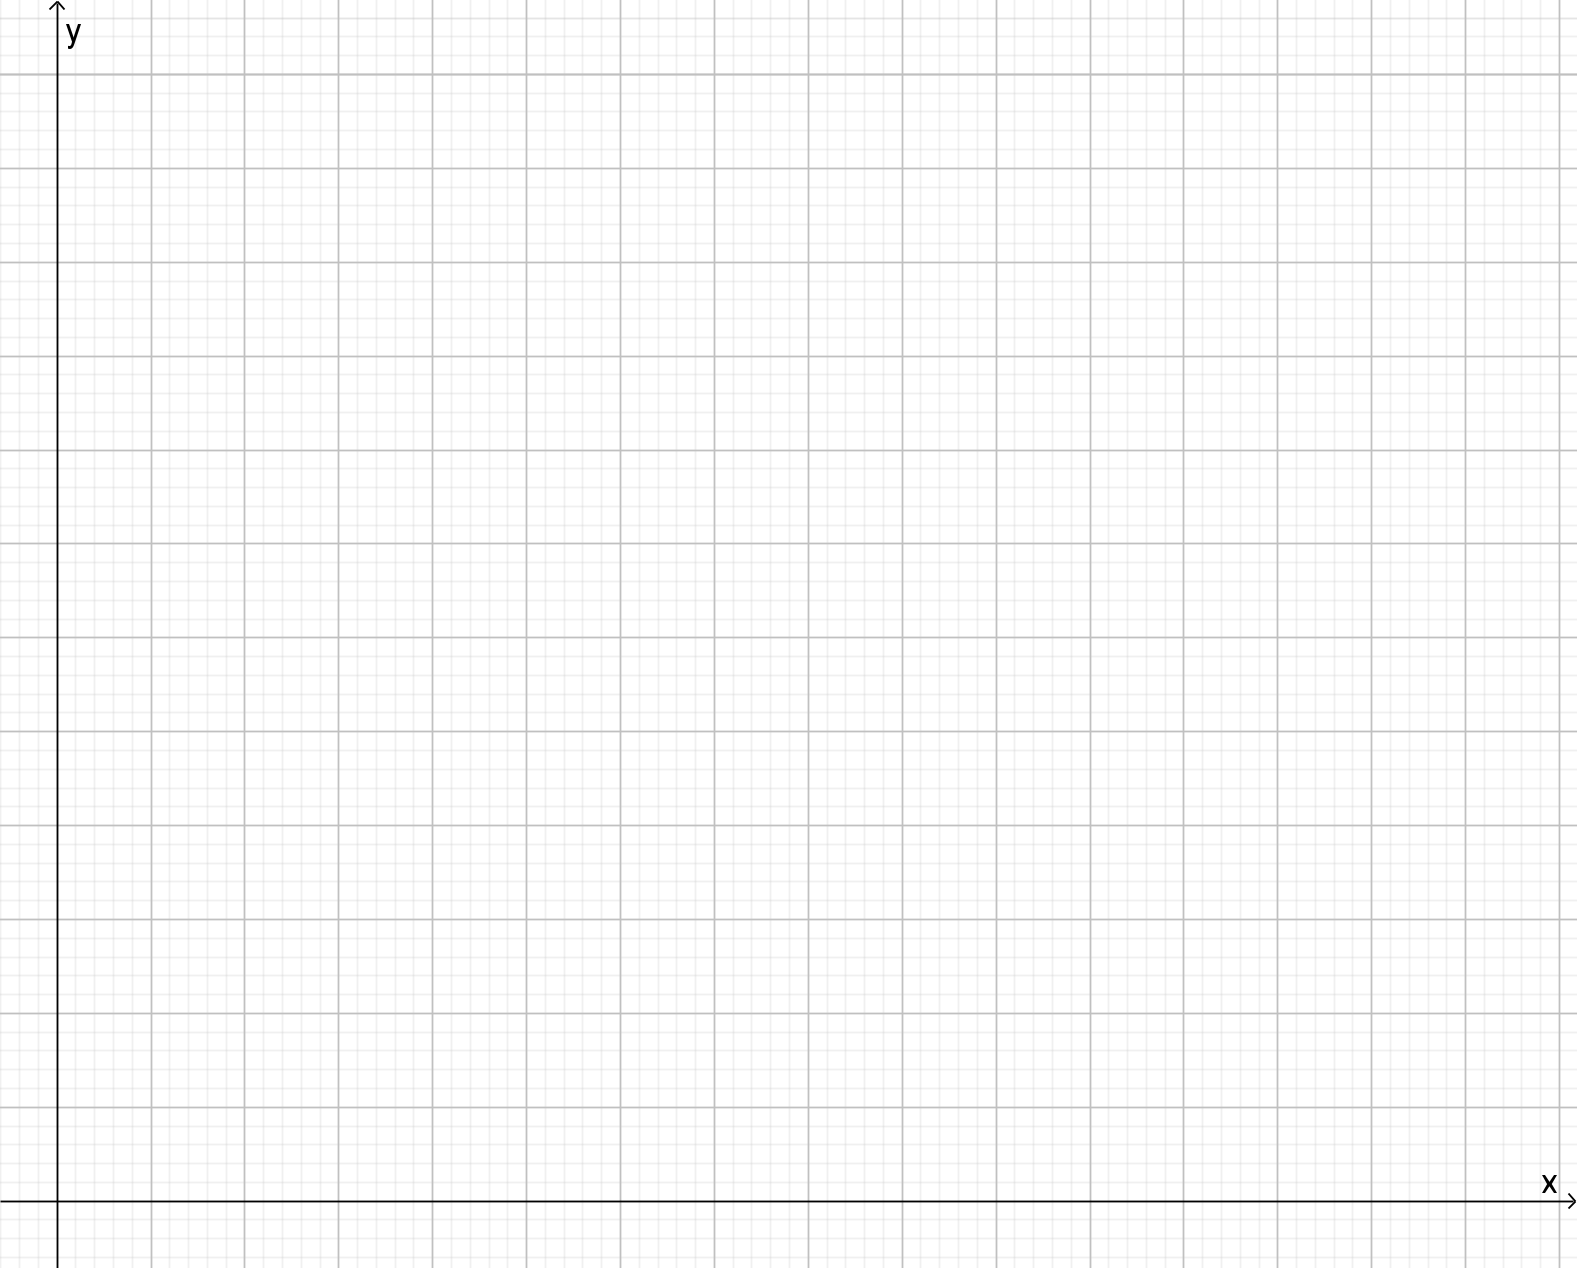
\includegraphics[width=0.86\textwidth]{../99_Bilder/KoordLeer.png}\\
			
\includegraphics[width=0.35\textwidth]{../../empty.jpg}
		\end{framed}
		\newpage
		
		%Blatt 3
		\setcounter{page}{1}
		\noindent
		\LARGE Labor\\
		\normalsize
		\noindent
		\begin{tabularx}{\textwidth}{Xr}
			\noindent
			Hewlett-Packard möchte ein Schullabor aufbauen, in dem Schüler arbeiten und lernen können. Neben den Schülern sollen auch Professoren hier arbeiten. Dabei bekommen Schüler ein Gehalt von \(6.000\)\euro{} und Professoren werden für ihre Betreuungsleistung mit \(10.000\)\euro{} bezahlt.& 
\includegraphics[width=0.15\textwidth,align=b]{../99_Bilder/comp.jpg}\\
			Insgesamt stehen \(230.000\)\euro{} für Gehaltszahlungen zur Verfügung.\\
			Jeder Professor kann aber nur 6 Schüler betreuen.\\			
		\end{tabularx}
		\begin{framed}
			\noindent
			\small{\color{codegray}Leitfrage:}\\
			
\includegraphics[width=0.1\textwidth]{../../empty.jpg}\\
		\end{framed}
		\begin{framed}
			\noindent
			\small{\color{codegray}Berechnung:}\\
			
\includegraphics[width=0.75\textwidth]{../../empty.jpg}
		\end{framed}
		\normalsize
		\newpage
		\begin{framed}
			\noindent
			\begin{tabularx}{\textwidth}{Xr}
				Der Vorstand eines Tennisvereins will für das kommende Jahr neue Mitgliedsbeiträge festlegen.Insgesamt muss der Verein aus den Mitgliedsbeiträgen \(28.800\)\euro{} einnehmen. & \multirow{2}{*}{
\includegraphics[width=0.15\textwidth,align=b]{../99_Bilder/sporty.jpg}}\\
				Im Verein sind \(120\) erwachsene und \(50\) jugendliche Mitglieder. & \\
				Der Vorstandsvorsitzende besteht darauf, dass Jugendliche ein Drittel von dem bezahlen, was Erwachsenen berechnet wird.\\
			\end{tabularx}\\
			\par\noindent
			Ermitteln Sie die Mitgliedsbeiträge für Jugendliche und Erwachsene!
		\end{framed}
		\begin{framed}
			\noindent
			\small{\color{codegray}Leitfrage:}\\
			
\includegraphics[width=0.1\textwidth]{../../empty.jpg}\\
		\end{framed}
		\begin{framed}
			\noindent
			\small{\color{codegray}Berechnung:}\\
			
\includegraphics[width=0.75\textwidth]{../../empty.jpg}
		\end{framed}
		\newpage
		
		%Blatt 4
		\setcounter{page}{1}
		\noindent
		\LARGE Handytarife\\
		\normalsize
		\noindent
		\begin{tabularx}{\textwidth}{Xl}
			\noindent
			Für das iPhone X liegen folgende Angebote vor: & \multirow{4}{*}{
\includegraphics[width=0.08\textwidth]{../99_Bilder/iphox.png}}
		\end{tabularx}
		\begin{tabularx}{\textwidth}{|l|l|l|}
			\cline{1-3}
			& Angebot klarmobil & Angebot Vodafone\\
			\cline{1-3}
			Einmalige Kosten & \(239\)\euro{} & \(109\)\euro{}\\
			\cline{1-3}
			monatliche Kosten & \(45\)\euro{} & \(52\)\euro{}\\
			\cline{1-3}
		\end{tabularx}
		\begin{framed}
			\noindent
			\small{\color{codegray}Leitfrage:}\\
			
\includegraphics[width=0.1\textwidth]{../../empty.jpg}\\
		\end{framed}
		\begin{framed}
			\noindent
			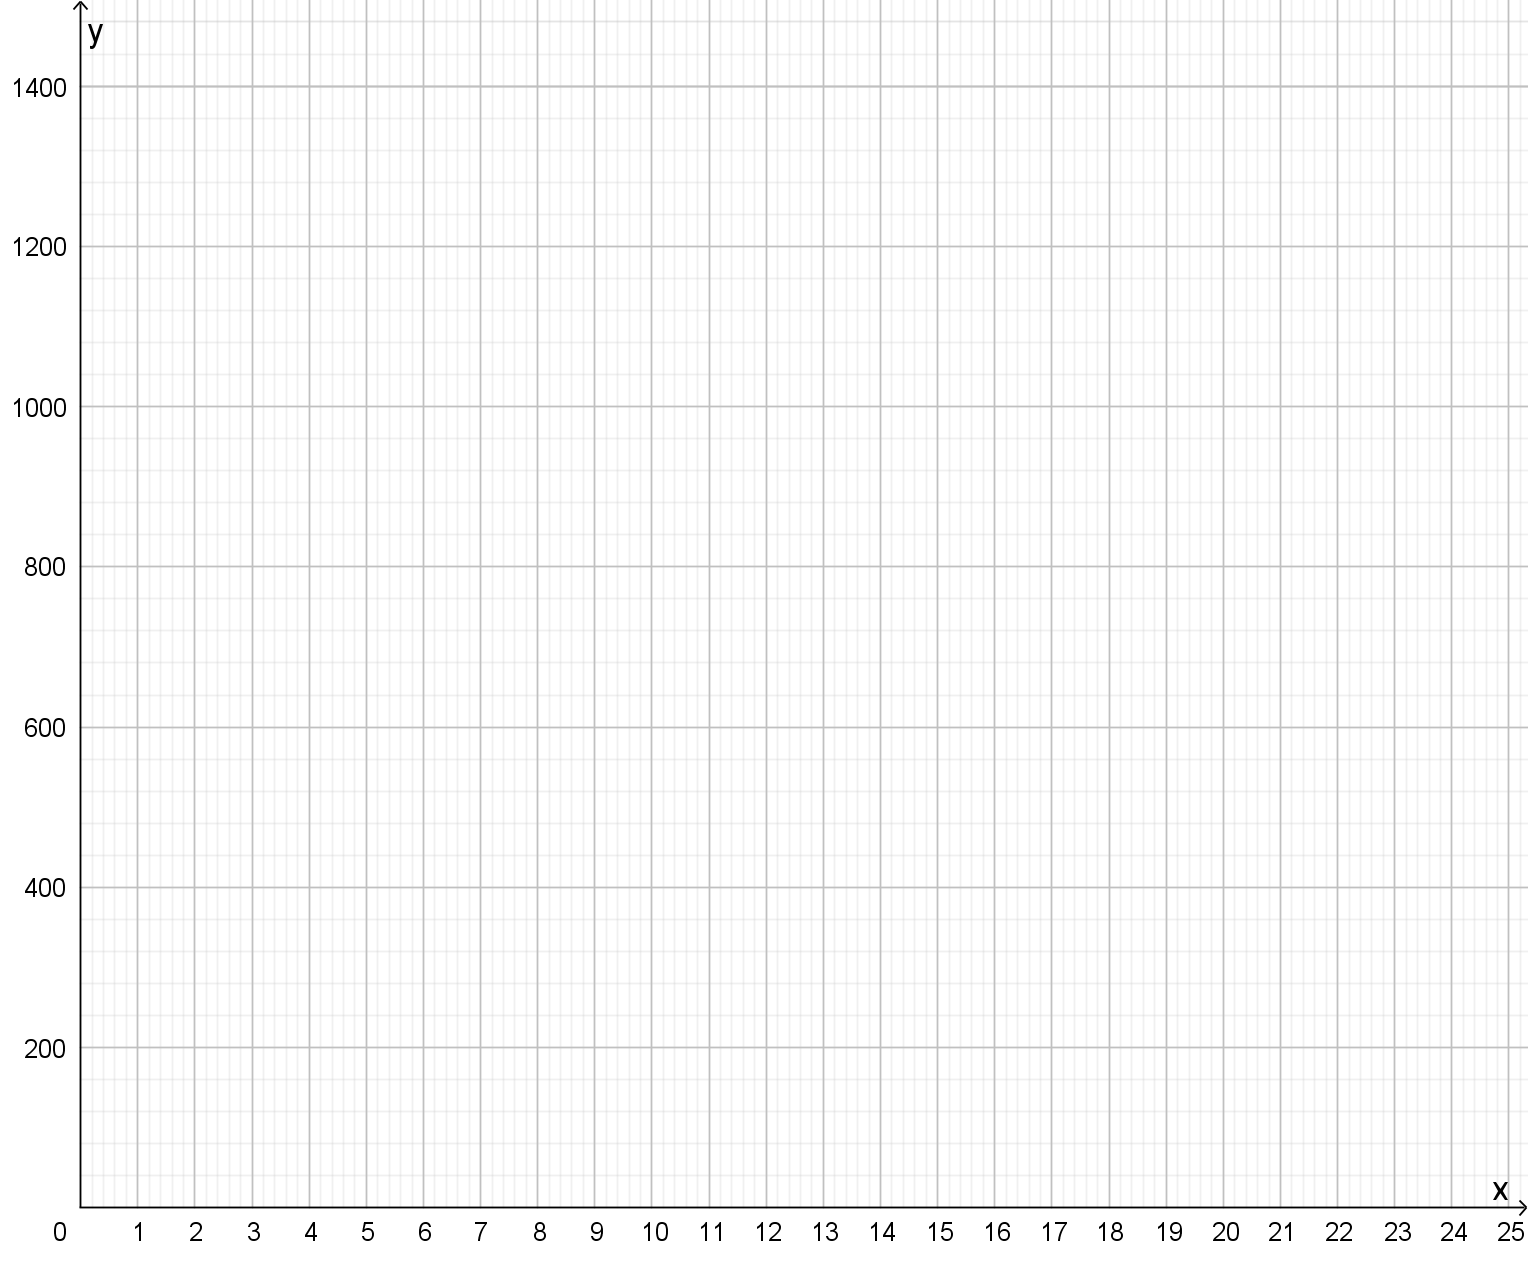
\includegraphics[width=0.6\textwidth]{../99_Bilder/KoordLeerSkal.png}\\
			\small{\color{codegray}Berechnung:}\\
			\begin{tabularx}{\textwidth}{X|L{3cm}|}
				\cline{2-2}
				
\includegraphics[width=0.2\textwidth]{../../empty.jpg} & Bringen Sie folgenden Pfeil im Koordinatensystem an: \includegraphics[width=0.1\textwidth,align=t]{../99_Bilder/arrow.png}\\
				&\\
				\cline{2-2}
			\end{tabularx}
			\par\bigskip\noindent
			\textbf{Entscheidung mit Begründung:}\\
			
\includegraphics[width=0.08\textwidth]{../../empty.jpg}
		\end{framed}
		\normalsize
		\newpage
		\begin{framed}
			\noindent
			\begin{tabularx}{\textwidth}{Xr}
				Die Wiesbadener Verkehrsgesellschaft bietet für ihren Radverleih die folgenden Tarife an:\\
				\begin{centering}
					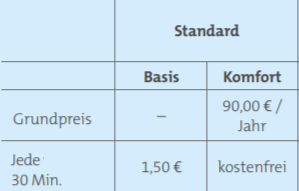
\includegraphics{../99_Bilder/eswe.png}
				\end{centering}
			\end{tabularx}
			\begin{itemize}
				\item[(a)] Stellen Sie zu beiden Angeboten die Funktionsgleichung auf.
				\item[(b)] Skizzieren Sie die Graphen der beiden Funktionen.
				\item[(c)] Bestimmen Sie, wann sich welches Angebot lohnt!
			\end{itemize}
		\end{framed}
		\begin{framed}
			\noindent
			\small{\color{codegray}Berechnung:}\\
			
\includegraphics[width=0.2\textwidth]{../../empty.jpg}\\
			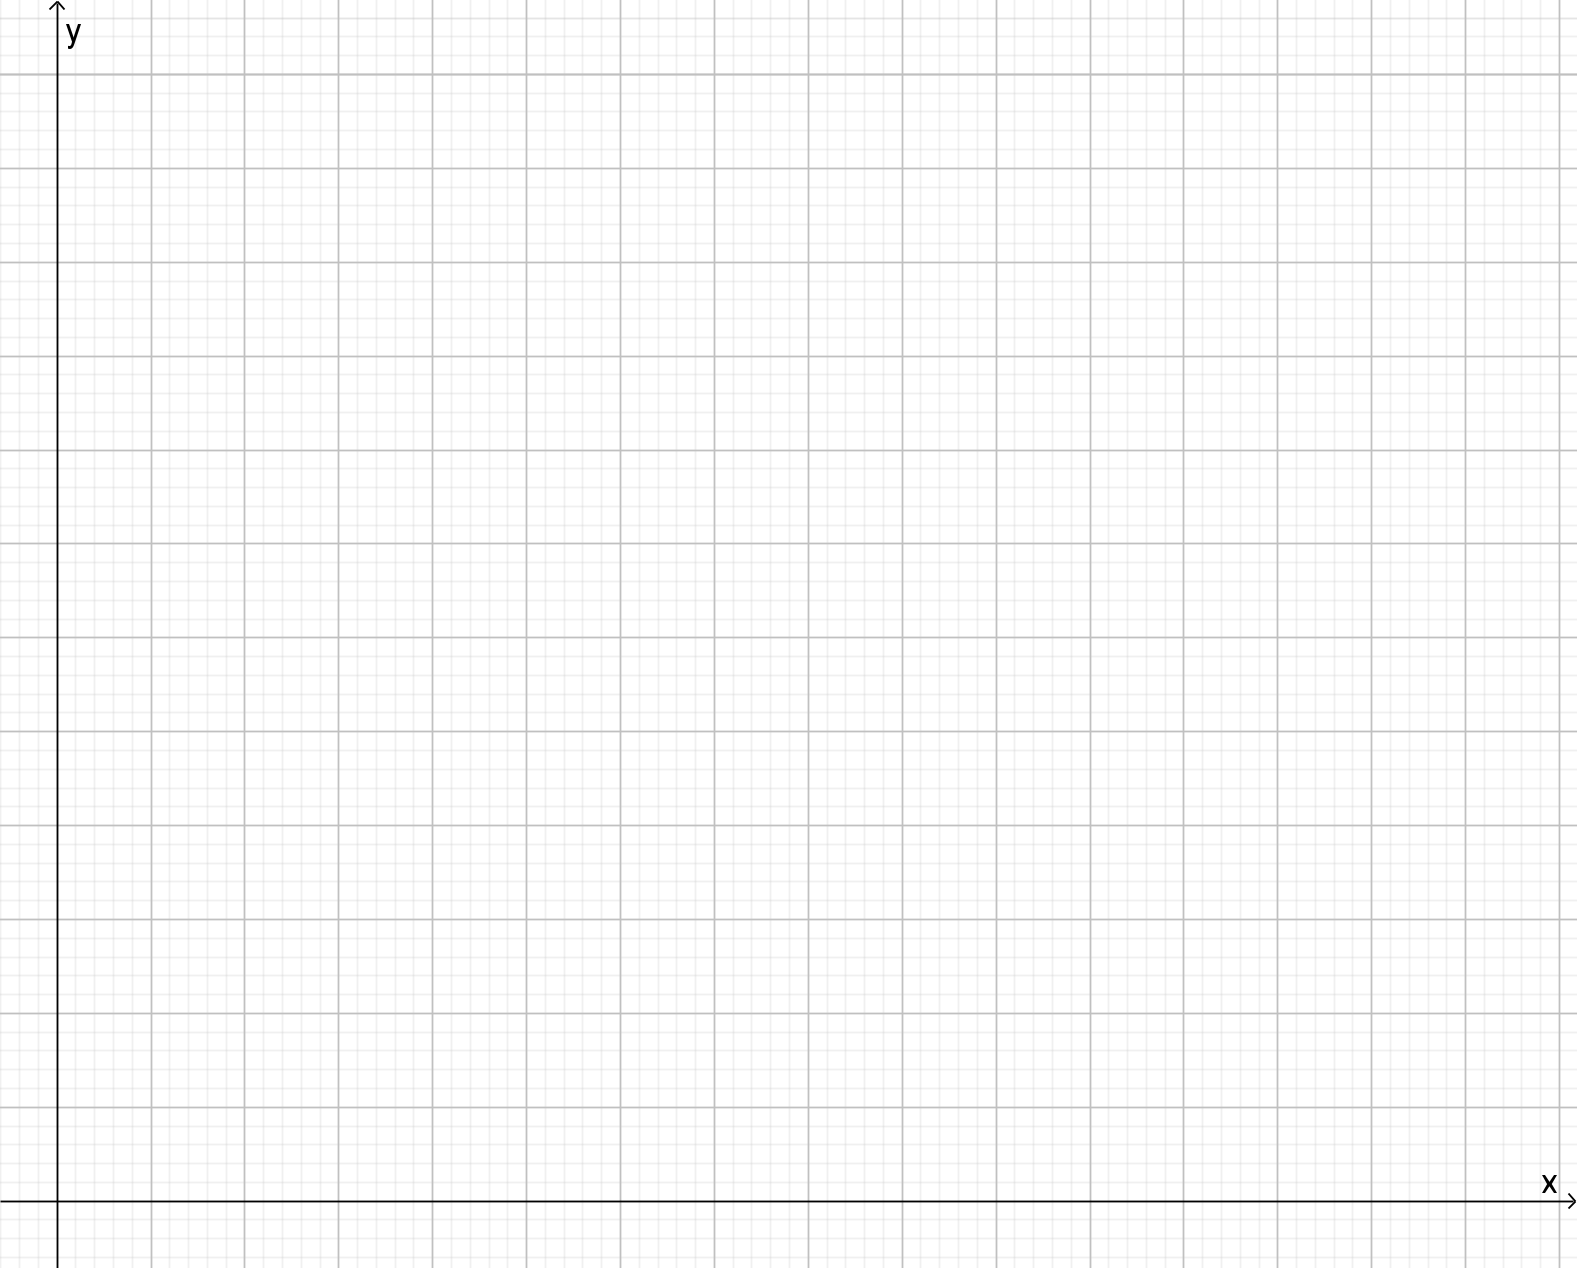
\includegraphics[width=0.8\textwidth]{../99_Bilder/KoordLeer.png}
		\end{framed}
	\end{worksheet}
\end{document}